\documentclass[10pt]{article}
\usepackage[margin=0.9in]{geometry}
\usepackage{graphicx}
\usepackage{booktabs}
\usepackage{amsmath}
\usepackage{caption}
\usepackage{subcaption}
\usepackage[hidelinks]{hyperref}
\usepackage{float}
\captionsetup{font=small}
\setlength{\parskip}{4pt}
\setlength{\parindent}{0pt}

\title{\vspace{-2.5em}Recovering Hidden Fire from RGB: Classical Deformable Models
vs.\ Deep Methods on FLAME-3}
\author{CS269 Project --- Deformable Models}
\date{\today}

\begin{document}
\maketitle
\vspace{-1.5em}

\section{Problem and Experimental Setup}

We study wildfire segmentation on the \textbf{FLAME-3} Fire subset (Sycan Marsh
aerial captures): 622 spatially aligned RGB/thermal frame pairs at
$512\times640$. The segmentation target is \emph{where the fire actually is
thermally}: the ground-truth (GT) mask is the paired radiometric thermal frame
thresholded at $\ge 150\,^\circ$C, followed by a $3\times3$ morphological
open/close and a 20-px minimum-blob filter. Thermal is used \emph{only} to
define the label; every method receives \textbf{RGB only} as its image input.

This framing is the crux of the experiment. In these captures the fire is
typically \emph{not} visible as orange flame in RGB---it is obscured by smoke.
We measured the red--green opponency ($R\!-\!G$, the canonical ``fire is red''
cue) and found in-fire pixels are no redder than background (mean
$R\!-\!G\approx2.5$ in-fire vs.\ $1.9$ background). A trivial color rule therefore
\emph{cannot} solve this task by construction; the question is whether a
deformable contour or a learned model can recover a largely hidden hot region.

\paragraph{Methods compared.} Two classical deformable models---\textbf{Kass
Snakes} (parametric, single closed contour; \texttt{skimage.active\_contour})
and \textbf{Geodesic Active Contours (GAC)} (morphological level set,
multi-component)---are run on the $R\!-\!G$ ``fire energy'' image. Both are
evaluated under two initialisations: \emph{oracle} (contour seeded from the GT
mask scaled outward $\sim$15\%, i.e.\ a known-location prior it only refines) and
\emph{color} (seeded from the $R\!-\!G$ color floor, no oracle). Three deep
baselines take RGB only and are trained against the same thermal masks:
\textbf{U-Net} (per-pixel CNN, the control), \textbf{DALS} (U-Net trunk + a
differentiable Chan--Vese level-set evolution), and \textbf{Deep Snake}
(circular-convolution contour deformation with detector-free coarse-seg
seeding). A \textbf{color floor} ($R\!-\!G$ threshold, no model, no init) is the
trivial reference.

\paragraph{Protocol.} Classical methods are scored on the 592 frames with
non-empty GT (30 empty-GT frames are skipped). Deep methods use a contiguous
70/15/15 train/val/test split (\texttt{flame/splits.py}) to avoid temporal
leakage between near-duplicate consecutive frames, and are scored on the
94-frame test split. All scores are IoU and Dice on binary masks at native
resolution. Deep models were trained 50 epochs each on an RTX 4090 (Adam,
$\text{lr}=10^{-4}$); checkpointed at best validation IoU.

\section{Quantitative Results}

Table~\ref{tab:main} and Figure~\ref{fig:bars} give the headline comparison.

\begin{table}[H]
\centering
\small
\begin{tabular}{llrrrrr}
\toprule
Method & Init & $n$ & mean IoU & med IoU & mean Dice & med lat (s) \\
\midrule
GAC        & oracle & 592 & \textbf{0.365} & 0.415 & 0.499 & 0.402 \\
Kass       & oracle & 592 & 0.198 & 0.179 & 0.305 & 0.277 \\
U-Net      & learned (RGB) & 94 & 0.147 & 0.037 & 0.207 & 0.003 \\
DALS       & learned (RGB) & 94 & 0.122 & 0.045 & 0.182 & 0.004 \\
Deep Snake & learned (RGB) & 94 & 0.032 & 0.000 & 0.032 & 0.003 \\
Color floor& none & 592 & 0.004 & 0.000 & 0.007 & 0.002 \\
GAC        & color & 592 & 0.003 & 0.000 & 0.006 & 0.418 \\
Kass       & color & 592 & 0.001 & 0.000 & 0.002 & 0.290 \\
\bottomrule
\end{tabular}
\caption{Mean/median IoU, mean Dice, and median per-frame latency.
Classical: 592 non-empty-GT frames; deep: 94-frame test split.}
\label{tab:main}
\end{table}

\begin{figure}[H]
\centering
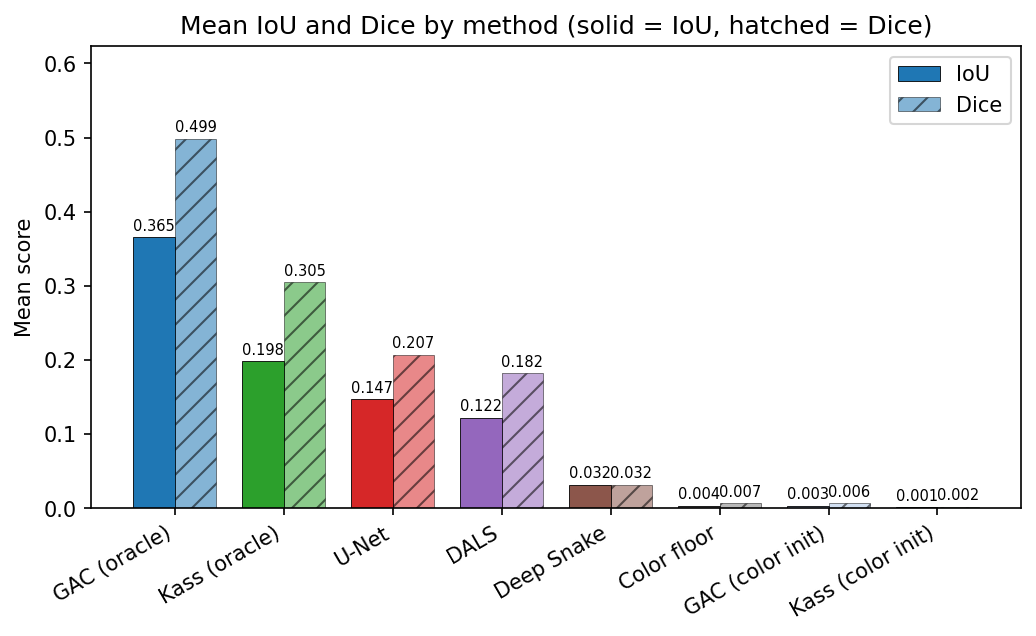
\includegraphics[width=0.78\textwidth]{figs/fig_bars.png}
\caption{Mean IoU (solid) and Dice (hatched) by method. The oracle contour
methods lead; the three RGB-only deep methods sit above the color floor; the
no-oracle contour methods collapse onto the floor.}
\label{fig:bars}
\end{figure}

\paragraph{Distributions, not just means.} The means hide a crucial difference
in \emph{shape}, shown in Figure~\ref{fig:box}. Oracle-GAC has mean
$\approx$ median ($0.365$ vs.\ $0.415$): it scores moderately on most frames. The
deep methods are the opposite---U-Net's mean ($0.147$) is far above its median
($0.037$), and Deep Snake's median is $0.000$. They succeed on a minority of
frames (where the fire happens to leave an RGB signature) and score near zero on
the rest, producing a heavy right tail rather than uniform competence.

\begin{figure}[H]
\centering
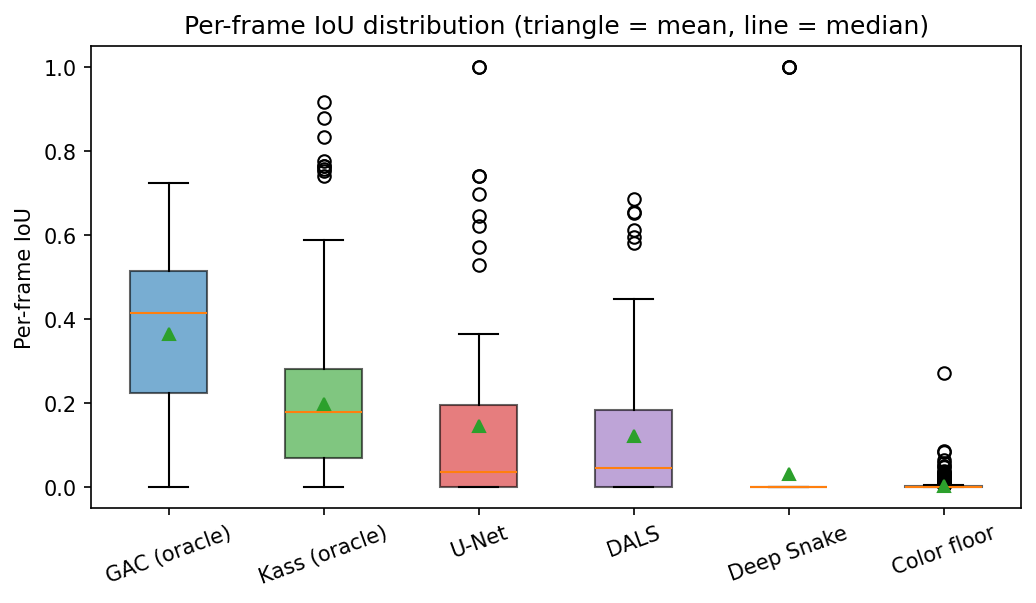
\includegraphics[width=0.78\textwidth]{figs/fig_box.png}
\caption{Per-frame IoU distributions. Oracle methods occupy a broad central
band; deep methods are concentrated near zero with a high-scoring tail (means,
triangles, pulled well above medians).}
\label{fig:box}
\end{figure}

\paragraph{Robustness to the GT threshold.} A reasonable worry is that the
$150\,^\circ$C cutoff is arbitrary and drives the ranking. Re-deriving the GT at
120/150/200\,$^\circ$C (Figure~\ref{fig:thr}, no-oracle init) leaves every
no-training method flat and near zero. The color floor and color-init contours
are uninformative \emph{regardless} of threshold, so the central conclusion is
not a $150\,^\circ$C artifact.

\begin{figure}[H]
\centering
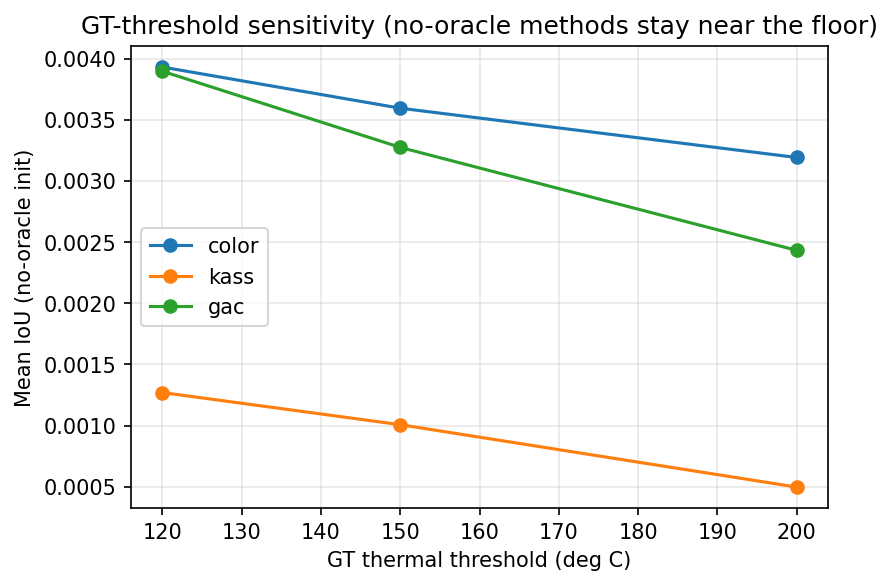
\includegraphics[width=0.55\textwidth]{figs/fig_threshold.png}
\caption{GT-threshold sensitivity (no-oracle init). All no-training methods stay
near the floor across 120--200\,$^\circ$C.}
\label{fig:thr}
\end{figure}

\section{Qualitative Input/Output Pairs}

For each method we show its best, median, and worst test frame by IoU. Cyan is
the thermal GT outline; magenta is the method's prediction. These make the
failure modes concrete.

\begin{figure}[H]
\centering
\begin{subfigure}{\textwidth}\centering
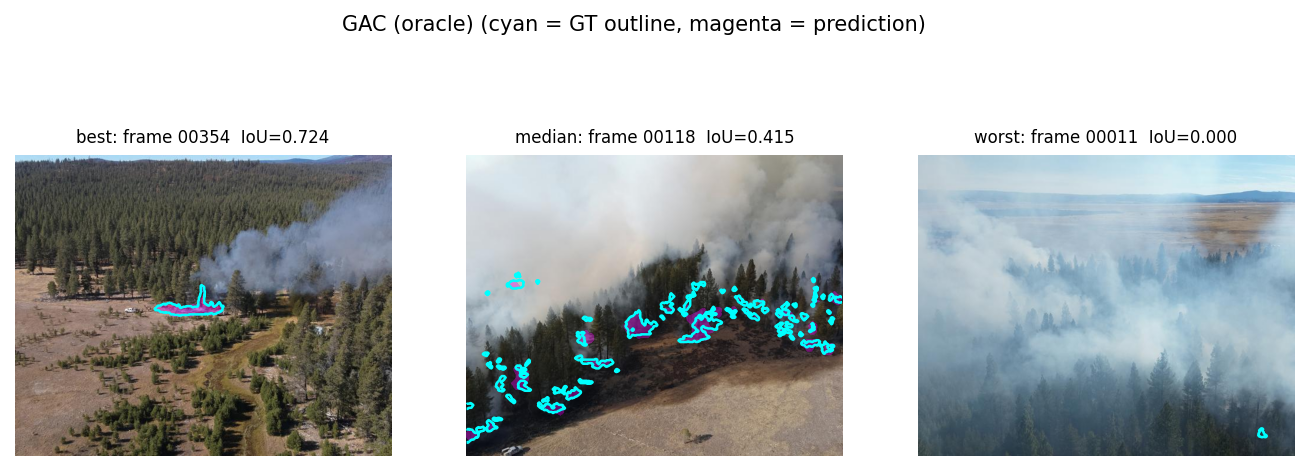
\includegraphics[width=\textwidth]{figs/fig_qual_gac_oracle.png}
\caption{\textbf{GAC (oracle).} Best case tightly recovers a compact front;
median over-grows along smoke gradients; worst is a frame where the fire is
fully smoke-occluded and the level set finds no boundary to lock onto (IoU 0).}
\end{subfigure}

\vspace{4pt}
\begin{subfigure}{\textwidth}\centering
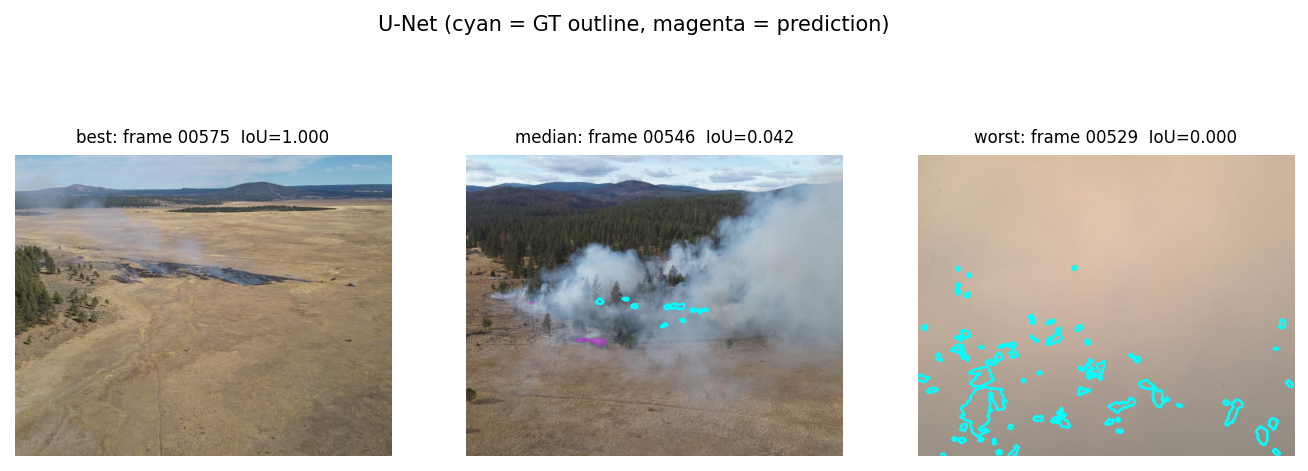
\includegraphics[width=\textwidth]{figs/fig_qual_unet.png}
\caption{\textbf{U-Net (RGB-only).} Best case localises the hot region from RGB
alone with no location prior---the key success the contour methods cannot
achieve without the oracle. Median/worst predict little or nothing where the
RGB carries no usable fire signature.}
\end{subfigure}
\caption{Qualitative best/median/worst pairs. Full set (Kass, DALS, Deep Snake,
color floor) in \texttt{report/figs/}.}
\label{fig:qual}
\end{figure}

\begin{figure}[H]
\centering
\begin{subfigure}{0.49\textwidth}\centering
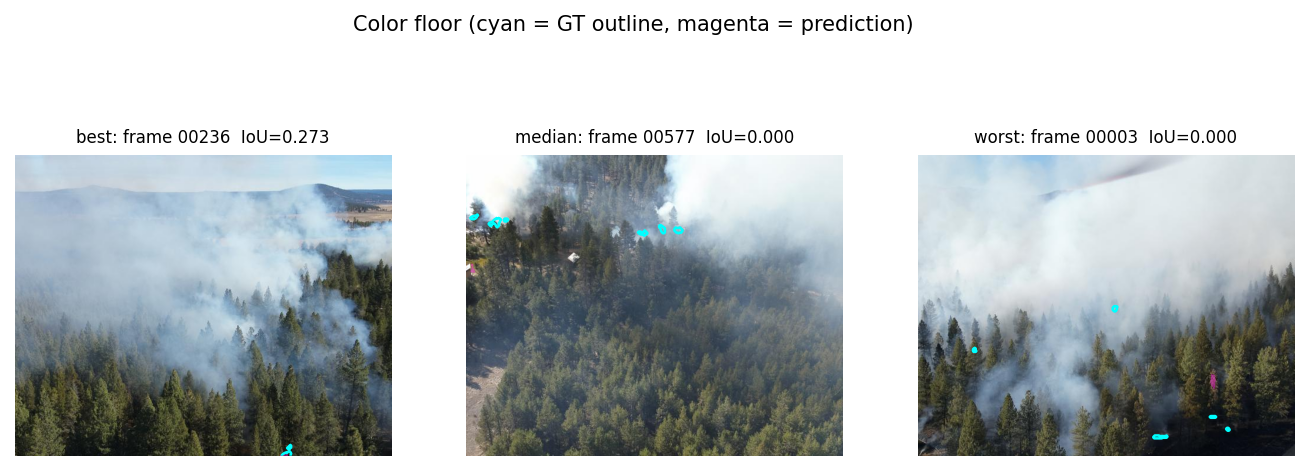
\includegraphics[width=\textwidth]{figs/fig_qual_color.png}
\caption{\textbf{Color floor.} Even its ``best'' frame barely overlaps GT---the
$R\!-\!G$ cue does not coincide with the thermal fire.}
\end{subfigure}\hfill
\begin{subfigure}{0.49\textwidth}\centering
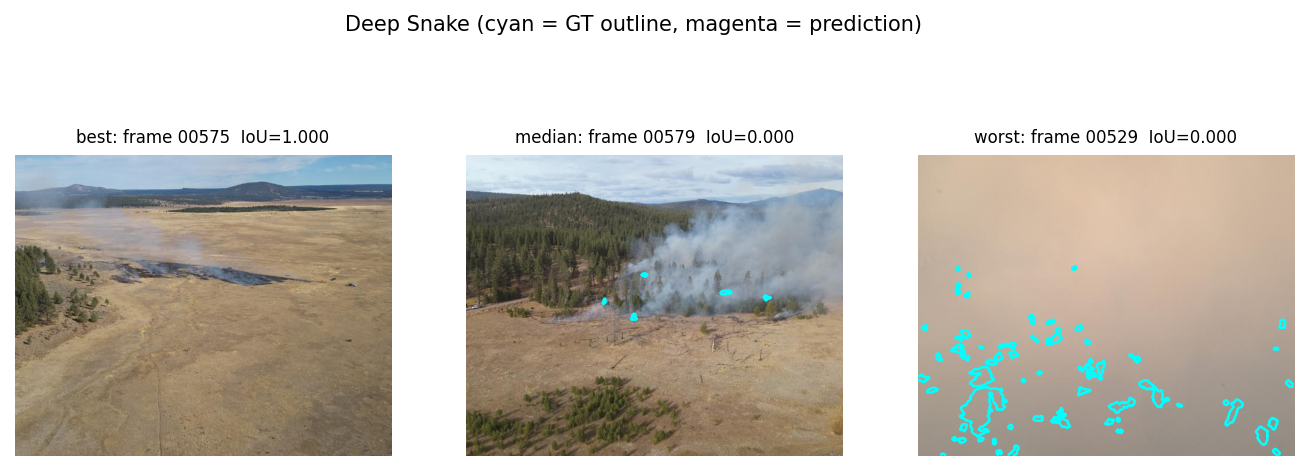
\includegraphics[width=\textwidth]{figs/fig_qual_deep_snake.png}
\caption{\textbf{Deep Snake.} Detector-free coarse-seg seeding is the weak
link: when the coarse head misses, no contour is initialised (median IoU 0).}
\end{subfigure}
\caption{The two extremes: the trivial color floor and the weakest deep method.}
\label{fig:qual2}
\end{figure}

\section{Conclusions}

\textbf{1. The color floor is $\approx$0; the task is genuinely hard.} At IoU
$0.004$ the $R\!-\!G$ rule confirms that thermal-defined fire is not recoverable
from RGB redness. This is a property of the data (smoke occlusion), not a tuning
failure, and it holds across GT thresholds.

\textbf{2. Oracle contours win the table but only \emph{refine} a handed-in
location.} GAC (0.365) and Kass (0.198) lead, but they are initialised from the
GT. Their strength is boundary refinement of a known region, not detection.

\textbf{3. Strip the oracle and the contour methods collapse to the floor}
(Kass 0.001, GAC 0.003). Seeded from the color prior instead of the GT, they have
no usable image gradient to evolve toward and fail completely. \emph{The
classical deformable models cannot \textbf{find} the fire from RGB---they can
only polish a boundary they are already given.}

\textbf{4. The RGB-only deep methods are the only ones that detect above the
floor without a prior.} U-Net (0.147) and DALS (0.122) sit an order of magnitude
above the color floor and the no-oracle contours, learning a faint RGB
signature of the hidden fire. They trail oracle-GAC, but that comparison is
apples-to-oranges: the deep methods receive \emph{no} location prior. Their
high-mean/low-median profile shows the capability is real but inconsistent---
strong on a minority of frames, near-zero on the rest.

\textbf{5. The contour \emph{head} did not help over a plain CNN.} DALS
(level-set head) and Deep Snake (contour head) did not beat the plain U-Net;
Deep Snake (0.032) underperformed because its detector-free coarse-seg seeding
fails whenever the coarse head misses the fire. On this data the bottleneck is
\emph{detection from a weak RGB cue}, which a per-pixel CNN handles at least as
well as a deformable head bolted on top.

\paragraph{Takeaway.} Deformable models are excellent boundary refiners but poor
detectors when the image cue is weak; the fair, prior-free comparison is won by
the learned per-pixel model. The honest framing of this result is detection from
a hidden cue, and under that framing the contour machinery's value is conditional
on a good initialisation it cannot supply itself.

\paragraph{Limitations / next steps.} Deep methods saw 50 epochs on a single
split; a fair contour-vs-CNN verdict would benefit from cross-validation and a
detection front-end for Deep Snake. A natural follow-up is to seed the classical
methods from the \emph{U-Net} prediction (a learned, prior-free init) rather than
the oracle or the color floor---testing whether contour refinement adds anything
on top of a real detector.

\end{document}
